\documentclass[9pt,a4paper]{extarticle}

\usepackage{f1000_styles}

\usepackage{hyperref}

\usepackage[numbers]{natbib}

\usepackage{tcolorbox} % for \texttt{}

\usepackage{bbding} % for \CheckmarkBold

% include \verb macros in \caption of figures

% http://tex.stackexchange.com/a/8814

\usepackage{cprotect}

\setlength{\parskip}{1ex}

\begin{document}

\pagestyle{front}

\title{CREATING AND SHARING REPRODUCIBLE RESEARCH CODE THE WORKFLOWR
WAY}

\author[1]{John D. Blischak}

\author[1,2]{Peter Carbonetto}

\author[1,3]{Matthew Stephens}

\affil[1]{Department of Human Genetics, University of Chicago}

\affil[2]{Research Computing Center, University of Chicago}

\affil[3]{Department of Statistics, University of Chicago}

\maketitle

\thispagestyle{front}

\begin{abstract}

% Note: Abstract can be as long as 300 words.

Making scientific analyses reproducible, well documented, and easily
shareable is crucial to maximizing their impact and ensuring that others
can build on them. However, accomplishing these goals is not easy,
requiring careful attention to organization, workflow, and familiarity
with tools that are not a regular part of every scientist's toolbox. We
have developed an R package, \textbf{workflowr}, to help all scientists,
regardless of background, overcome these challenges. \textbf{Workflowr} aims to
instill a particular ``workflow'' --- a sequence of steps to be repeated
and integrated into research practice --- that helps make projects more
reproducible and accessible.This workflow integrates four key elements:
(1) version control (via \textbf{Git}); (2) literate programming (via R
Markdown); (3) automatic checks and safeguards that improve code
reproducibility; and (4) sharing code and results via a browsable
website. These features exploit powerful existing tools, whose mastery
would take considerable study. However, the \textbf{workflowr} interface is
simple enough that novice users can quickly enjoy its many benefits. By
simply following the \textbf{workflowr} ``workflow'', R users can create projects
whose results, figures, and development history are easily accessible on
a static website --- thereby conveniently shareable with collaborators
by sending them a URL --- and accompanied by source code and
reproducibility safeguards. The \textbf{workflowr} R package is open source and
available on CRAN, with full documentation and source code available at
\url{https://github.com/jdblischak/workflowr}.

\end{abstract}

\section*{Keywords}

reproducibility, open science, workflow, R, interactive programming,
literate programming, version control

\clearpage

\pagestyle{main}


\section*{Introduction}

A central tenet of the scientific method is that results should be
independently verifiable --- and, ideally, extendible --- by other
researchers. As computational methods play an increasing role in many
disciplines, key scientific results are often produced by computer code.
Verifying and extending such results requires that the code be
``reproducible''; that is, it can be accessed and run, with outputs that
can be corroborated against published results \cite{Buckheit1995,
Gentleman2007, Peng2011, Ince2012, Morin2012, Sandve2013,
Easterbrook2014, Stodden2016, Lowndes2017}. Unfortunately, this ideal is
not usually achieved in practice; most scientific articles do not come
with code that can reproduce their results \cite{Ioannidis2009,
Merali2010, Ioannidis2014, Stodden2018}.

There are many barriers to sharing reproducible code and corresponding
computational results \cite{kitzes2017}. One barrier is simply that
keeping code and results sufficiently organized and documented is
difficult --- it is burdensome even for experienced programmers who are
well-trained in relevant computational tools such as version control
(discussed later), and even harder for the many domain scientists who
write code with little formal training in computing and informatics
\cite{Wilson2014}. Further, modern interactive computer environments
(e.g., R, Python), while greatly enhancing code development
\cite{Findler2002}, also make it easier to create results that are
irreducible. For example, it is all too easy to run interactive code
without recording or controlling the seed of a pseudo-random number
generator, or generate results in a ``contaminated'' environment that
contains objects whose values are critical but unrecorded. Both these
issues can lead to results that are difficult or impossible to
reproduce. Finally, even when analysts produce code that is reproducible
in principle, sharing it in a way that makes it easy for others to
retrieve and use (e.g., via GitHub or Bitbucket) involves technologies
that many scientists are not familiar with \cite{Marwick2017,
Stodden2018}.

In light of this, there is a pressing need for easy-to-use tools to help
analysts maintain reproducible code, document progress, and disseminate
code and results to collaborators and to the scientific community. We
have developed an open source R \cite{R2019} package, \textbf{workflowr}, to
address this need. The \textbf{workflowr} package aims to instill a particular
``workflow'' --- a sequence of steps to be repeated and integrated into
research practice --- that helps make projects more reproducible and
accessible. To achieve this, \textbf{workflowr} integrates four key features that
facilitate reproducible code development: (1) version control
\cite{Loeliger2012, Chacon2014}; (2) literate programming
\cite{Xie2018}; (3) automatic checks and safeguards that improve code
reproducibility; and (4) sharing code and results via a browsable
website. These features exploit powerful existing tools, whose mastery
would take considerable study. However, the \textbf{workflowr} interface is
designed to be simple so that learning it does not become another
barrier in itself and novice users can quickly enjoy its many benefits.
By simply following the \textbf{workflowr} ``workflow'', R users can create
projects whose results and figures are easily accessible on a static
website --- thereby conveniently shareable with collaborators by sending
them a URL --- and accompanied by source code and reproducibility
safeguards. The Web-based interface, updated with version control, also
makes it easy to navigate through different parts of the project and
browse the project history, including previous versions of figures and
results, and the code used to produce them. By using \textbf{workflowr}, all this
can be achieved with minimal experience in version control systems and
Web technologies.

The \textbf{workflowr} package builds on several software technologies and R
packages, without which this work would have been impossible. \textbf{Workflowr}
builds on the invaluable R Markdown literate programming system
implemented in \textbf{knitr} \cite{Xie2014, knitrpkg} and \textbf{rmarkdown}
\cite{Xie2018, rmarkdownpkg}, which in turn build on \textbf{pandoc}, the
``Markdown'' markup language, and various Web technologies such as
Cascading Style Sheets and Bootstrap \cite{Spurlock2013}. Several
popular R packages extend \textbf{knitr} and \textbf{rmarkdown} for specific aims such as
writing blogs  (\textbf{blogdown} \cite{blogdown}), monographs  (\textbf{bookdown}
\cite{bookdown}), and software documentation  (\textbf{pkgdown} \cite{pkgdown}).
Analogously, \textbf{workflowr} extends \textbf{rmarkdown} with additional features such
as the reproducibility safeguards, and adds integration with the version
control system \textbf{Git} \cite{Loeliger2012, Chacon2014}. \textbf{Git} was designed to
support large-scale, distributed software development, but in \textbf{workflowr}
it serves a different purpose: to record, and provide access to, the
development history of a project. \textbf{Workflowr} also uses another feature of
 \textbf{Git}, ``remotes'', to enable collaborative project development across
multiple locations, and to help users create browsable projects via
integrations with popular online services such as GitHub Pages and
GitLab Pages. These features are implemented using the R package \textbf{git2r}
\cite{git2r}, which provides an interface to the \textbf{libgit2} C library.
Finally, beyond extending the R programming language, \textbf{workflowr} is also
integrated with the popular \textbf{RStudio} interactive development environment
\cite{rstudio}.

In addition to the tools upon which \textbf{workflowr} directly builds, there are
many other related tools that directly or indirectly advance open and
reproducible data analysis. A comprehensive review of such tools is
beyond the scope of this article, but we note that many of these tools
are complementary to \textbf{workflowr} in that they tackle aspects of
reproducibility that \textbf{workflowr} currently leaves to the user, such as
management and deployment of computational environments and dependencies
(e.g., \textbf{conda}, \textbf{Homebrew}, \textbf{Singularity}, \textbf{Docker}, \textbf{Kubernetes}, \textbf{packrat}
\cite{packrat}, \textbf{checkpoint} \cite{checkpoint}, \textbf{switchr} \cite{switchr},
 \textbf{RSuite} \cite{rsuite}); development and management of computational
pipelines (e.g., \textbf{GNU Make}, \textbf{Snakemake} \cite{snakemake}, \textbf{drake}
\cite{drake}); management and archival of data objects (e.g., \textbf{archivist}
\cite{archivist}, Dryad \cite{dryad}, Zenodo); and distribution of open
source software (e.g., CRAN, Bioconductor \cite{bioconductor}, Bioconda
\cite{bioconda}). Most of these tools or services could be used in
combination with \textbf{workflowr}. There are additional, ambitious efforts to
develop cloud-based services that come with many computational
reproducibility features (e.g., Code Ocean, Binder, Gigantum, The Whole
Tale). Many of these platforms manage individual projects as \textbf{Git}
repositories, so \textbf{workflowr} could, in principle, be installed and used on
these platforms, possibly to enhance their existing features. Other R
packages with utilities to facilitate reproducibility that could
complement \textbf{workflowr} include \textbf{ProjectTemplate} \cite{projecttemplate},
 \textbf{rrtools} \cite{rrtools}, and \textbf{usethis} \cite{usethis}, as well as many of
the R packages listed in the ``Reproducible Research'' CRAN Task View
(https://CRAN.R-project.org/view=ReproducibleResearch).

Of the available software tools facilitating reproducible research,
perhaps the closest in scope to \textbf{workflowr} are the R package \textbf{adapr}
\cite{Gelfond2018} and the Python-based toolkit \textbf{Sumatra}
\cite{Davidson2014}. Like \textbf{workflowr}, both \textbf{adapr} and \textbf{Sumatra} use version
control to maintain a project development history. Unlike \textbf{workflowr},
both place considerable emphasis on managing and documenting
dependencies (software and data), whereas \textbf{workflowr} only records this
information. In contrast, \textbf{workflowr} places more emphasis on literate
programming --- the publishing of text and code in a readable form ---
and more closely integrates other features such as tracking project
development history via \textbf{Git} with literate programming.

The \textbf{workflowr} R package is available from CRAN
(https://cran.r-project.org/package=workflowr) and GitHub
(https://github.com/jdblischak/workflowr), and is distributed under the
flexible open source MIT license. The R package and its dependencies are
straightforward to install while being highly customizable for more
dedicated users. Extensive documentation, tutorials, and user support
can be found at the GitHub site. In the remainder of this article, we
describe the \textbf{workflowr} interface, explain its design, and give examples
illustrating how \textbf{workflowr} is used in practice.


\section*{Operation}

In this section, we give an overview of \textbf{workflowr}'s main features from a
user's perspective. For step-by-step instructions on starting a
 \textbf{workflowr} project, see the
\href{https://jdblischak.github.io/workflowr/articles/wflow-01-getting-started.html}{``Getting
started with \textbf{workflowr}''} vignette.

For basic usage, only five functions are needed (summarized here, and
described in more detail later):

\begin{itemize}

\item \texttt{wflow\_start()} initializes a new project, including the template
directory structure (Figure \ref{fig:organized}A);

\item \texttt{wflow\_build()} renders webpages from R Markdown (Rmd) analysis
files, with reproducibility safeguards in place;

\item \texttt{wflow\_publish()} renders the webpages and updates the project
development history—it commits the code, calls \texttt{wflow\_build()}, then
commits the webpages;

\item \texttt{wflow\_status()} reports the status of the project files; and

\item \texttt{wflow\_git\_push()} uploads the results from the user's local
repository to a website hosting service.

\end{itemize}

\textit{The primary output of \textbf{workflowr} is a project website for
browsing the results generated by the Rmd analysis files} (Figure \ref{fig:organized}B).
The use of websites to organize information is, of course, now
widespread. Nonetheless, we believe they are under-utilized for
organizing the results of scientific projects. In particular, hypertext
provides an ideal way to connect different analyses that have been
performed, and to provide easy access to relevant external data (e.g.,
related work or helpful background information); see Figure \ref{fig:organized}B and ``Use
cases'' below.

\subsection*{Organizing the project: \texttt{wflow\_start()}}



\begin{figure}

% Figure \ref{fig:organized}

\centering

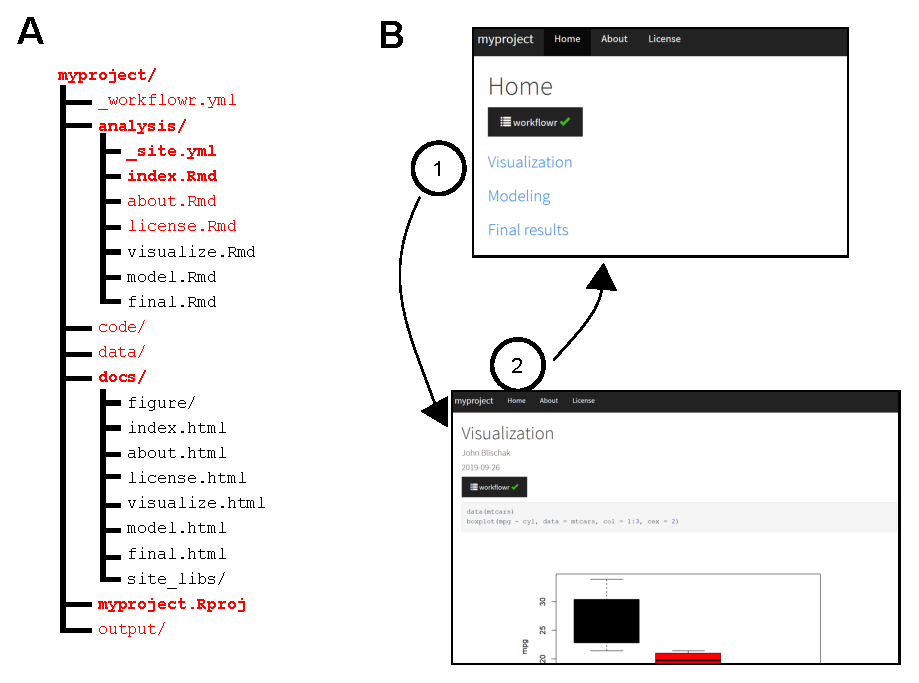
\includegraphics[width=0.8\textwidth]{figures/wflow-fig-1-v03.eps}

\cprotect\caption{\label{fig:organized}

The \textbf{workflowr} package helps organize project files and results. A) The
function \texttt{wflow\_start()} populates a project directory with all the files
and subdirectories (shown in red) needed to begin a \textbf{workflowr} project.
This default directory structure encourages users to organize their
files as the project progresses—as the project develops, additional Rmd
files may be organized in the "analyses" folder. (This is only a
suggested structure; users can change the names of most files and
directories. Required files are shown in boldface.) B) All results are
organized into a website (all HTML files generated by \textbf{workflowr} are
automatically stored in \texttt{docs/}). The use of hyperlinks allows
for efficient access to the results. The screenshots above illustrate
how a \textbf{workflowr} website can be navigated. Clicking a hyperlink in the
main page, \texttt{index.html}, (1) navigates the browser to a webpage
containing some results, \texttt{visualize.html}; clicking on the
``Home'' hyperlink (2) in the navigation bar brings the browser back to
the main page. For larger projects, the navigation bar can be used to
quickly access different sections of a project.

}

\end{figure}

The function \texttt{wflow\_start()} facilitates project organization by
populating a directory with suggested subdirectories, scripts, and
configuration files for a data analysis project (Figure \ref{fig:organized}A). The
subdirectories created by default are \texttt{analysis/}, where the Rmd
analysis files are stored; \texttt{docs/}, which stores the website HTML
files; \texttt{code/}, which is intended for longer-running scripts,
compiled code (e.g., C++) and other source code supporting the data
analyses; \texttt{data/}, for storing raw data files; and \texttt{output/},
for saving processed data files and other outputs generated by the
scripts and analyses. This setup is flexible and configurable; only two
of the directories, \texttt{analysis/} and \texttt{docs/}, are required, and
both can be renamed later.

In addition to creating a default file structure for a data analysis
project, \texttt{wflow\_start()} also initializes the project development history:
it creates a \textbf{Git} repository, and commits the files and directories to
this repository. This is all done behind the scenes so no familiarity
with \textbf{Git} is needed. We give more details about the \textbf{Git} repository in the
``Implementation'' section below.

In some cases, a user will have an existing project (with files that may
or may not be tracked by \textbf{Git}), and would like to incorporate \textbf{workflowr}
into the project --- \texttt{wflow\_start()} also easily accommodates this
scenario, with additional arguments to control how the \textbf{workflowr} files
are added to the existing project. See the package vignette, ``Migrating
an existing project to use \textbf{workflowr},'' for more details; it can be
accessed by running vignette("wflow-03-migrating") after loading the
 \textbf{workflowr} package in R.

Finally, \texttt{wflow\_start()} changes R’s working directory to the root of the
project directory. Although this is a simple step, it is important for
correctly resolving file paths. Forgetting to change the working
directory is a very common source of errors in data analyses.

\subsection*{Generating results reproducibly: \texttt{wflow\_build()}}

In a \textbf{workflowr} project, analyses are performed using the R Markdown
literate programming system \cite{Xie2018}. The user develops their R
code inside Rmd files in the \texttt{analysis/} directory, then calls
\texttt{wflow\_build()}, which runs the code and renders the results as HTML files
in the \texttt{docs/} directory. The \texttt{wflow\_build()} function extends the
\texttt{render\_site()} command from the \textbf{rmarkdown} package with several
reproducibility safeguards:

1. It creates a clean R session for executing the code. This is critical
for reproducibility—results should not depend on the current state of
the user's R environment, and all objects necessary to run the code
should be defined in the code or loaded by packages.

2. It automatically sets the working directory in a consistent manner
(the exact setting is controlled by a configuration file; see
``Implementation'' below). This prevents one of the most common failures
to reproduce in R—not setting the working directory before running the R
script, resulting in incorrectly resolved relative file paths.

3. It sets a seed for the pseudorandom number generator before executing
the code. This ensures that analyses that use random numbers always
return the same result.

4. It records information about the computing environment, including the
operating system, the version of R used, and the packages that were used
to produce the results.

Finally, \texttt{wflow\_build()} summarizes the results of these reproducibility
safeguards in a report at the top of the webpage, along with additional
``reproducibility checks'' which alert the user to potential
reproducibility issues, such as changes that were not committed to the
project development history, and the use of (non-reproducible) absolute
file paths (Figure \ref{fig:reproducible}).

\subsection*{Keeping track of the project's development: \texttt{wflow\_publish()}}

As a project progresses, many versions of the results will be generated
as results are scrutinized, analyses are revised, errors are corrected,
and new data are considered. Keeping track of a project's evolution is
important for documenting progress and retracing the development of the
analyses. This is sometimes done without version control tools by
copying code and results whenever an important change is made. This
typically results in a large collection of files with names such as
\texttt{results-v2-final\_final.pdf} or
\texttt{anova\_analyses\_before\_adding\_new\_samples.R}. This approach
is tedious and error-prone, and makes it difficult to communicate
changes to collaborators.

The version control system, \textbf{Git}, provides a more systematic and reliable
way to keep track of a project's development history. However, \textbf{Git} was
designed to manage source code for large-scale software projects, and
using it for scientific analyses brings some specific challenges. The
relative complexity of \textbf{Git} provides a high barrier to entry,
discouraging many researchers from adopting it for their projects. And
 \textbf{Git} is not ideally suited to data analysis projects where one wants to
coordinate the tracking of source code, data, and \textit{the results
generated by the code and data}. Using \textbf{Git} commands to identify the
version of the code that was used to generate a result can be
non-trivial.

The \texttt{wflow\_publish()} function is designed to address these challenges: it
takes the steps necessary to coordinate tracking of code and results,
and reduces these steps to calling a single, easy-to-use function. The
command performs three steps, detailed in Figure \ref{fig:publish}. These steps are
designed to ensure that each new collection of results added to the
project development history has been produced by a unique and
identifiable version of an Rmd analysis file.

Even experienced \textbf{Git} users will benefit from using \texttt{wflow\_publish()}.
Besides the convenience of a single function, \texttt{wflow\_publish()} ensures
that:

\begin{enumerate}

\item Every commit to an (Rmd) analysis file is associated with a commit
to the results file generated by that analysis file.

\item \textit{An analysis file is only published and committed if it
runs successfully}; on failure, \texttt{wflow\_publish()} aborts, and neither code
nor results are committed to the \textbf{Git} repository. (R code that does not
work can still be committed to a \textbf{workflowr} project via other methods,
e.g., directly using \textbf{Git}, but it will not be associated with a committed
results file.)

\end{enumerate}



\begin{figure}

% Figure \ref{fig:publish}

\centering

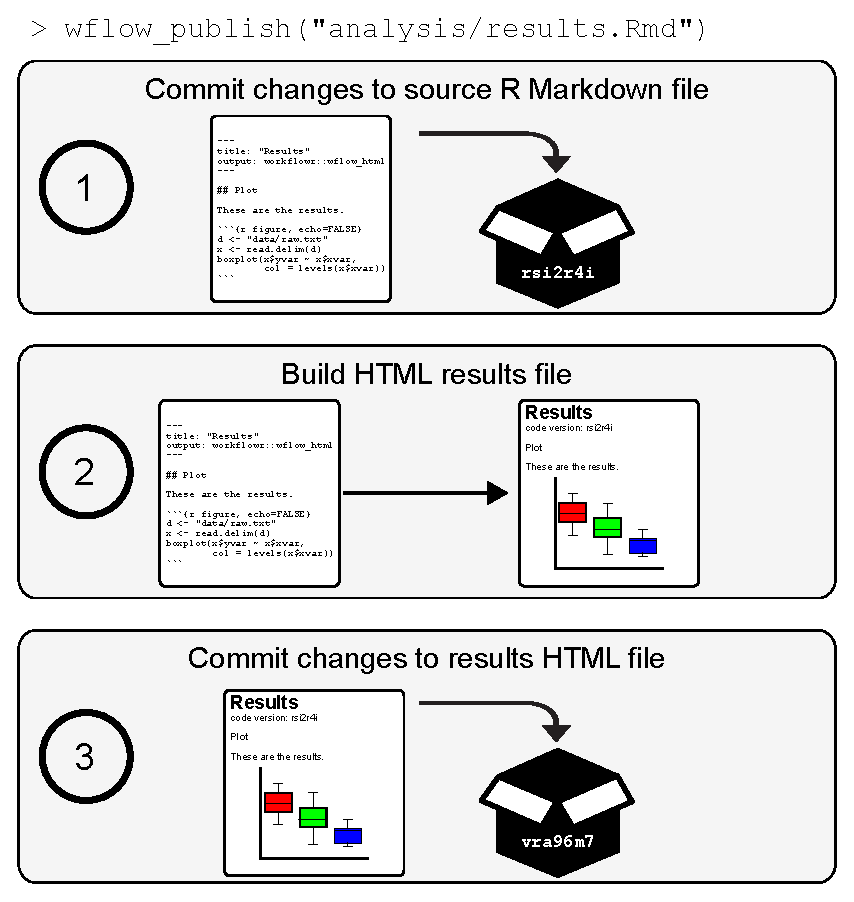
\includegraphics[width=0.8\textwidth]{figures/wflow-fig-2-v03.eps}

\cprotect\caption{\label{fig:publish}

The function \texttt{wflow\_publish()} simplifies and coordinates tracking of the
source code and results files in a \textbf{Git} repository. The function performs
a 3-step procedure to store the code and results in a project
development history, and ensure that the result HTML file is always
created from a unique and identifiable versioned Rmd analysis file. (1)
The first step commits the changes to the Rmd analysis file. (2) The
second step builds the results HTML file from the Rmd file. These two
steps ensure that the results were generated from the committed version
of the Rmd file. Furthermore, the unique version of the \textbf{Git} repository
is inserted directly into the HTML file so that the source code used to
generate the results is easily identified and accessed. If the code
generates an error, the entire process is aborted and the previous
commit made in the first step is undone. (3) The results HTML file, as
well as any related figure files, are committed to the \textbf{Git} repository.
Thus, the versioning of Rmd analysis files and corresponding HTML
results files are coordinated whenever \texttt{wflow\_publish()} is used.

}

\end{figure}

Publishing an analysis is not necessarily final --- after calling
\texttt{wflow\_publish()}, the analysis can be repeatedly updated and re-published
using \texttt{wflow\_publish()}. Each time \texttt{wflow\_publish()} succeeds in committing
a new version of the code and results, a link to previously published
versions of the analysis are embedded in the webpage so that readers can
easily access previous versions and compare with the latest results.

\subsection*{Checking in on the project's development: \texttt{wflow\_status()}}

As a \textbf{workflowr} project grows, it is important to be able to get an
overview of the project's status and identify files that may need
attention. This functionality is provided by the \texttt{wflow\_status()} command,
which gives the status of each Rmd file in the project --- either
“scratch”, “unpublished”, or “published”, whose definitions are given in
Figure \ref{fig:versioned}. The “published” Rmd files, which are those that have been run
through \texttt{wflow\_publish()}, are further recorded as either “up-to-date” or
“modified” depending on whether the Rmd file has been modified since
\texttt{wflow\_publish()} was run. The \texttt{wflow\_status()} function highlights all Rmd
files in the ``scratch'', ``unpublished'' or ``modified'' states, and
suggests suitable next steps.



\begin{figure}

% Figure \ref{fig:versioned}

\centering

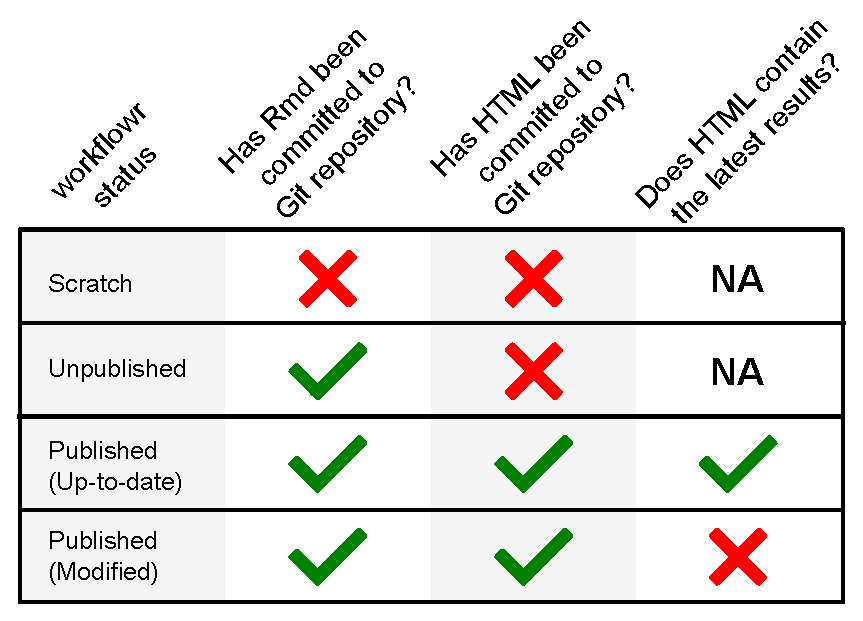
\includegraphics[width=0.8\textwidth]{figures/wflow-fig-3-v02.eps}

\cprotect\caption{\label{fig:versioned}

The \textbf{workflowr} package is an R Markdown-aware version control system. The
function \texttt{wflow\_status()} assigns a state to each Rmd file in the
 \textbf{workflowr} project based on its status in the \textbf{Git} repository's working
tree, and based on the \textbf{Git} status of the associated HTML results file.

}

\end{figure}



\begin{figure}

% Figure \ref{fig:reproducible}

\centering

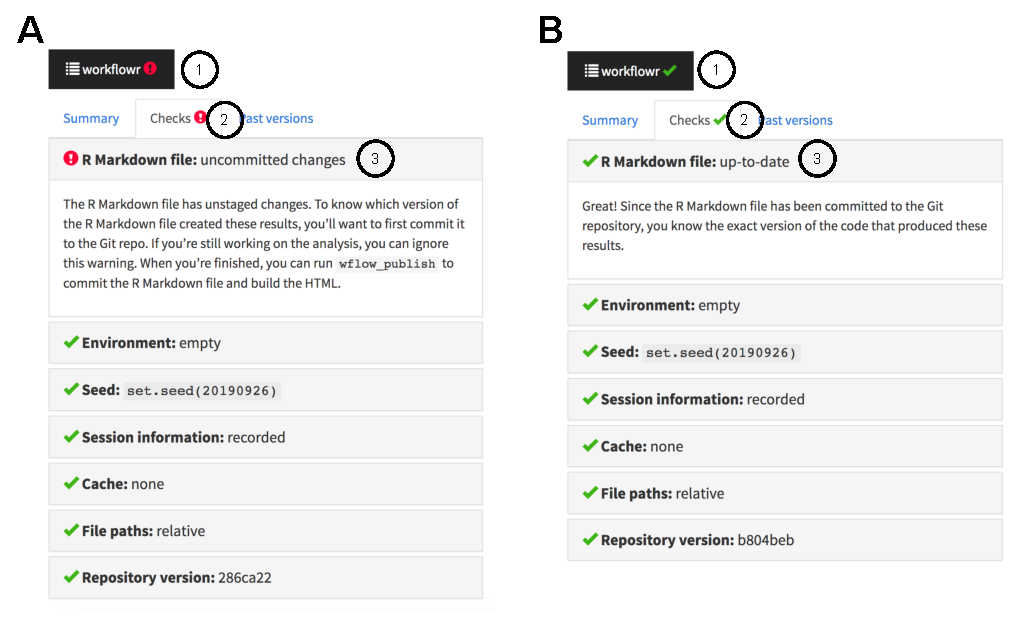
\includegraphics[width=0.8\textwidth]{figures/wflow-fig-4-v02.eps}

\cprotect\caption{\label{fig:reproducible}

The \textbf{workflowr} reproducibility report summarizes the reproducibility
checks inside the results webpage. (A) A button is added to the top of
each webpage. Clicking on the button (1) reveals the full
reproducibility report with multiple tabs. If any of the reproducibility
checks have failed, a red warning symbol (!) is shown. Clicking on the
"Checks" tab (2) summarizes the reproducibility checks, with icons next
to each check indicating a pass or failure. Clicking on an individual
item (3) reveals a more detailed description of the reproducibility
check, with an explanation of why it passed or failed. In (A), the Rmd
file contains changes that have not yet been committed, so one of the
reproducibility checks has failed. (Uncommitted changes are acceptable
during active development, but not acceptable when results are
published.) In this case, the recommendation is given to run
\texttt{wflow\_publish()} to fix the issue. (B) If all the \textbf{workflowr}
reproducibility checks pass, the \textbf{workflowr} button shows a green
checkmark (\CheckmarkBold), and clicking an individual item in the
reproducibility report (3) gives more detail on the reproducibility
check.

}

\end{figure}

\subsection*{Sharing code and results: \texttt{wflow\_git\_push()}}

The version-controlled website created by \textbf{workflowr} is self-contained,
so it can be hosted by most Web servers with little effort. Once the
website is available online, the code and results can be shared with
collaborators and colleagues by providing them with the website's URL.
Similarly, the \textbf{workflowr} repository can also serve as a companion
resource for a manuscript by referencing the website URL in the paper.

Since a \textbf{workflowr} project is also a \textbf{Git} repository, the most convenient
way to make the website available online is to use a \textbf{Git} hosting
service. The \textbf{workflowr} package includes functions \texttt{wflow\_use\_github()} and
\texttt{wflow\_use\_gitlab()} to simplify the setup process on two of the most
widely used services, GitHub and GitLab. Once a user has created a \textbf{Git}
repository on one of these online platforms, the project can be easily
uploaded using \texttt{wflow\_git\_push()}. (There is also a companion function
\texttt{wflow\_git\_pull()} which is used when multiple people are collaborating on
a \textbf{workflowr} project, or when a project is being updated from multiple
computers.)

The results files in a \textbf{workflowr} website include links to past versions
of analysis and figures, making it easy for collaborators to benefit
from the versioning of analyses without knowing anything about \textbf{Git}. For
example, if a collaborator wants to download a previous version of a
figure generated several months ago, this can be done by navigating the
links on the \textbf{workflowr} website.

\subsection*{Installation}

The \textbf{workflowr} package is available on CRAN. It works with R versions
2.3.5 or later, and can be installed on any major platform that is
supported by R (Linux, macOS, Windows). It is regularly tested on all
major operating systems via several Continuous Integration services
(AppVeyor, CircleCI, Travis CI). It is also regularly tested by CRAN
using machines running Debian GNU/Linux, Fedora, macOS, Solaris, and
Windows.

Because \textbf{workflowr} uses the \textbf{rmarkdown} package to build the HTML pages, it
requires the document conversion software \textbf{pandoc} to be installed. The
easiest way for R users to install \textbf{pandoc} is to install \textbf{RStudio}.
Installing \textbf{Git} is not required because the R package dependency \textbf{git2r}
includes \textbf{libgit2}, a minimal \textbf{Git} implementation. (Nonetheless, installing
 \textbf{Git} may be useful for occasional management of the \textbf{Git} repository
outside regular \textbf{workflowr} usage.)

\subsection*{Customization}

 \textbf{Workflowr} projects are highly customizable. For example, the look of the
webpages can be customized, via options provided by the \textbf{rmarkdown}
package, by editing the \texttt{analysis/\_site.yml} configuration file.
Additional settings specific to \textbf{workflowr}, such as setting the seed for
the pseudorandom number generator, or setting the working directory for
the Rmd files, can be controlled in the \texttt{\_workflowr.yml} file.


\section*{Implementation}

Here we give an overview of the \textbf{workflowr} package implementation. All \textbf{workflowr} commands can be invoked from R (or \textbf{RStudio}) so long as the working directory in R is set to the directory containing a \textbf{workflowr} project, or any subdirectory of a \textbf{workflowr} project (this is similar to how \textbf{Git} commands are invoked). To determine the root directory of a \textbf{workflowr} project from a subdirectory, whenever a command is called from the R console, \textbf{workflowr} uses the \textbf{rprojroot} \cite{rprojroot} R package to search for the \textbf{RStudio} project file stored at the root of the project. (The \textbf{RStudio} project file is a required file, so if this file is deleted, the \textbf{workflowr} commands will not work.)

\subsection*{Organizing the project: \texttt{wflow\_start()}}

The function \texttt{wflow\_start()} populates the project directory using
predefined template files (see Figure \ref{fig:organized}). It uses the \textbf{glue} \cite{glue} R
package to insert relevant variables, e.g., the name of the project,
directly into the newly created files. When \texttt{wflow\_start()} is called with
\texttt{git = TRUE} (which is the default), a \textbf{Git} repository is created
in the project directory, and all newly created or modified files are
committed to the repository. If the user has never previously created a
 \textbf{Git} repository on their computer they may need to first call
\texttt{wflow\_git\_config()} to configure \textbf{Git}.

\subsection*{Generating results reproducibly: \texttt{wflow\_build()}}

The \texttt{wflow\_build()} function generates a responsive website from a
collection of Rmd files. Both \texttt{wflow\_build()} and \texttt{wflow\_publish()} support
file patterns, also known as “wildcard expansion”; for example,
\texttt{wflow\_build("analysis/*.Rmd")} will generate webpages for all
the Rmd files in the \texttt{analysis/} directory.

The \texttt{wflow\_build()} function extends the \texttt{render\_site()} function from the
 \textbf{rmarkdown} package. The \texttt{render\_site()} function in turn builds on the
Bootstrap framework to create a responsive website with a navigation
bar. This rendering step includes downloading and linking to the
required CSS and JavaScript files. Many website settings, such as the
labels and URLs included in the navigation bar, can be adjusted in the
\texttt{analysis/\_site.yml} configuration file. (These options can also
be set individually inside the Rmd files, which will override the
default options set in \texttt{analysis/\_site.yml}. ) Like other R
packages that extend \textbf{rmarkdown} (e.g., \textbf{bookdown}), \textbf{workflowr} provides a
custom site generator in the function \texttt{wflow\_site()} which alters the
website generation process. For example, one change to this process is
that the generated website files (the HTML, CSS, JavaScript and figures)
are moved instead of copied from \texttt{analysis/} to \texttt{docs/}. This
reduces unnecessary duplication of files. Most of \textbf{workflowr}’s key
features, including the reproducibility report, are implemented in
\texttt{wflow\_html()}, which we describe next.

In the \textbf{rmarkdown} package, the rendering of individual webpages from Rmd
files is controlled by a separate function, \texttt{html\_document()}. The
 \textbf{workflowr} package provides an analogous function, \texttt{wflow\_html()}. This
function also extends \texttt{html\_document()}, so all features implemented in
 \textbf{rmarkdown} (e.g., code chunk folding, generating a table of contents from
the section headings) are inherited by \texttt{wflow\_html()}.

Most of the \textbf{workflowr} content is added as a preprocessing step prior to
executing the R code in the Rmd file. To achieve this, \texttt{wflow\_html()}
copies the original Rmd file to a temporary directory, incorporates the
additional content, then executes the code. The content embedded into
the Rmd file includes a code chunk that calls \texttt{set.seed()}, a code chunk
toward the end of the file that calls \texttt{sessionInfo()}, and inline HTML
tags for elements such as the reproducibility report and links to
previous versions of figures. There is also a brief postprocessing step
to incorporate additional HTML, CSS, and JavaScript elements needed to
display the \textbf{workflowr} elements added in the preprocessing step. This
postprocessing is done when \textbf{pandoc} converts the generated markdown to
the final webpage.

The process for embedding links to past versions of files --- that is,
files added to previous commits in a \textbf{Git} repository --- requires some
additional explanation. Links to past versions are included only if the
user has set up a remote repository hosted by either GitHub and GitLab.
Clicking on a link to a past version of an Rmd file (or figure file) in
a Web browser will load a webpage displaying the R Markdown source code
(or figure file) as it is saved in the given commit. For past versions
of the webpages, we use an independent service
\href{https://raw.githack.com/}{raw.githack.com}, which displays the
HTML file in the browser like any other webpage (this is because GitHub
and GitLab only show the raw HTML code). These links will point to valid
webpages only after the remote repository (on GitHub or GitLab) is
updated, e.g., using \texttt{wflow\_git\_push()}. In the current implementation,
when an Rmd file (and its corresponding HTML file) is renamed, the
webpage does not include links to past versions prior to renaming. So
renaming files will limit the ability to browse the project development
history.

The \texttt{wflow\_html()} function allows for considerable customization of the
 \textbf{workflowr} reproducibility report, and other features. The settings in
the \texttt{analysis/\_site.yml} configuration file are passed to
function \texttt{html\_document()} in the \textbf{rmarkdown} package, whereas the settings
in \texttt{\_workflowr.yml} are read by \texttt{wflow\_html()}; see
\texttt{help(wflow\_html)} for a full details on all \textbf{workflowr} settings
that can be customized in this file. For example, the default function
used to record the session information at the bottom of each webpage,
\texttt{sessionInfo()}, can be overridden by adding the YAML field
\texttt{sessioninfo} (e.g., the function from the \textbf{devtools}
\cite{devtools} package could be used instead by setting
\texttt{sessioninfo:\;devtools::session\_info()}).

To execute the code, \texttt{wflow\_build()} first creates a new R session to
execute the code. This is implemented using the R package \textbf{callr}
\cite{callr}.

By default, the \textbf{rmarkdown} package renders an Rmd file in the directory
where the Rmd file is stored; that is, the R working directory is
automatically changed to the directory containing the target Rmd file.
By default, \texttt{wflow\_html()} overrides the behaviour, and instead executes
the R code with respect to the root project directory. This default is
intended to improve reproducibility by resolving file paths from a
consistent reference point. This execution directory can be controlled
by the \texttt{knit\_root\_dir} option, which is set in the 
\texttt{\_workflowr.yml} configuration file. By default, new projects execute the
R Markdown code chunks in the root directory. If this setting is not
configured, \textbf{workflowr} reverts to the \textbf{rmarkdown} default. It is also
possible to have a different \texttt{knit\_root\_dir} setting for
different files, but this is generally not recommended as it will make
the code more difficult to follow.

\subsection*{Keeping track of the project's development: \texttt{wflow\_publish()}}

One of the steps in \texttt{wflow\_publish()}, as we have mentioned, is a call to
\texttt{wflow\_build()}. It also runs \textbf{Git} commands to commit the source code and
rendered HTML files (Figure \ref{fig:publish}). These \textbf{Git} commands are executed behind
the scenes. We have also implemented many checks and extensive error
handling to make sure that the \textbf{Git} repository and R environment are in
an acceptable state for committing the results. When an issue arises,
\texttt{wflow\_publish()} attempts to detect the issue as early as possible, then
it reverts the \textbf{Git} repository to the initial state and, when possible,
suggests how to fix the issue. For example, \texttt{wflow\_publish()} will stop if
any of the files contain conflicts from a previous merge using \textbf{Git}.

\subsection*{Checking in on the project's development: \texttt{wflow\_status()}}

The \texttt{wflow\_status()} function checks the status of each Rmd file in the
project by comparing the state of the file in the \textbf{Git} repository's
working tree against the \textbf{Git} status of the corresponding HTML file. In
 \textbf{Git} terminology, a “scratch” Rmd file in a \textbf{workflowr} project is an
uncommitted file in a \textbf{Git} repository; “unpublished” means that the Rmd
file is committed to the \textbf{Git} repository but the corresponding HTML is
not; a "published" Rmd file and its HTML file are both committed to the
 \textbf{Git} repository; and a "modified" Rmd file has changes --- these changes
can be unstaged, staged, or committed --- that were made since the last
time the corresponding HTML file was committed (Figure \ref{fig:versioned}).

Using \textbf{git2r}, it is mostly straightforward to determine the status of
each file. The only complicated step is determining whether published
Rmd files have been modified. If all changes to an Rmd file have been
committed to the \textbf{Git} history, an Rmd file is considered “modified” if it
has modifying commits that are more recent than commits modifying the
corresponding HTML file.

\subsection*{Sharing the code and results: \texttt{wflow\_git\_push()}}

To use \texttt{wflow\_git\_push()}, the remote \textbf{Git} repository must first be
configured. The user can configure the remotes manually using the
\texttt{git remote} subcommand or using \texttt{wflow\_git\_remote()}.
Alternatively, the \textbf{workflowr} package provides two functions,
\texttt{wflow\_use\_github()} and \texttt{wflow\_use\_gitlab()}, that simplify the creation
and configuration of remote repositories hosted on GitHub and GitLab.
These two convenience functions also add a navigation bar link with the
URL of the remote source code repository. The \texttt{wflow\_use\_gitlab()}
function takes the additional step of activating the GitLab Pages by
creating a file \texttt{.gitlab-ci.yml} with the proper configuration.
(GitHub Pages must be set up manually; there is currently no way to
automate this via the GitHub API.)


\section*{Use cases}

 \textbf{Workflowr} was officially released on CRAN in April 2018. As of September
2019, it has been downloaded from CRAN over 7,000 times, and it has been
adopted by many researchers. The most common use cases are 1)
documenting research development and including the project website in
the accompanying academic paper, and 2) developing reproducible course
materials to share with students. Here we highlight some successful
examples.

\subsection*{Repositories for research projects}

\textbf{Human dermal fibroblast clonality project}

\url{https://davismcc.github.io/fibroblast-clonality}

A \textbf{workflowr} project accompanying a scientific paper on computational
methods for decoding the clonal substructures of somatic tissues from
DNA sequencing data \cite{McCarthy2018}. The webpages describe how to
reproduce the data processing and analysis, along with the outputs and
plots.

\textbf{Characterizing and inferring quantitative cell cycle phase in
single-cell RNA-seq data analysis}

\url{https://github.com/jdblischak/fucci-seq}

A \textbf{workflowr} project supporting a paper on measuring cell cycle phase and
gene expression levels in human induced pluripotent stem cells
\cite{Hsiao2019}. The repository contains the processed data and the
code implementing the analyses. The full results can be browsed on the
website.

\textbf{Flexible statistical methods for estimating and testing effects
in genomic studies with multiple conditions}

\url{https://github.com/stephenslab/gtexresults}

A \textbf{workflowr} project containing the code and data used to produce the
results from the GTEx data set that were presented in \cite{Urbut2019}.

\textbf{Investigations on "truncated adaptive shrinkage"}

\url{https://github.com/LSun/truncash}

A \textbf{workflowr} project created by a Ph.D. student created to keep track of
his investigations into controlling false discoveries in the presence of
correlation and heteroskedastic noise. This repository illustrates the
use of \textbf{workflowr} as a scientific notebook --- the webpages contain
written notes, mathematical equations, source code, and the outputs
generated from running the code.

\subsection*{Repositories for courses}

\textbf{Stanford STATS 141—Biostatistics}

\url{https://xiangzhu.github.io/stanford-stats141}

A \textbf{workflowr} website for a Biostatistics course taught at Stanford. The
website includes working R examples, homework, the course syllabus, and
other course materials.

\textbf{Single-cell RNA-seq workshop}

\url{https://github.com/crazyhottommy/scRNA-seq-workshop-Fall-2019}

A \textbf{workflowr} website for a workshop on analysis of single-cell RNA-seq
data offered by the Harvard Faculty of Arts and Sciences Informatics
group as part of a two-week long bioinformatics course. The R examples
demonstrate how to use several bioinformatics packages such as \textbf{Seurat}
and \textbf{msigdbr} to prepare and analyze single-cell RNA-seq data sets.

\textbf{Introduction to GIS in R}

\url{https://github.com/annakrystalli/intro-r-gis}

A \textbf{workflowr} website for a workshop given at the 2018 Evolutionary
Biology Conference. The website includes working R demonstrations, setup
instructions, and exercises.


\section*{Summary}

Our main aim in developing \textbf{workflowr} is to lower barriers to open and
reproducible code. \textbf{Workflowr} provides a core set of commands that can be
easily integrated into research practice, and combined with other tools,
to make projects more accessible and reproducible. The R package is
straightforward to install, easy to learn, and highly customizable.

Since the first official release of \textbf{workflowr} (version 1.0.1, released
in April 2018), the core functionality has remained intact, and we
expect it to remain that way. The core features of \textbf{workflowr} have been
carefully tested and revised, in large part thanks to feedback and issue
reports from the user community. Our next aim is to implement several
enhancements, including:

\begin{itemize}

\item Create a centralized \textbf{workflowr} project website to make it easier
for researchers to share and discover \textbf{workflowr} projects.

\item Provide additional functions to simplify website hosting on other
popular platforms such as Netlify and Heroku.

\item As \textbf{workflowr} projects grow, it becomes increasingly important to
document not only the evolution of the code and results over time, but
also how the results interrelate with one another. Therefore, we aim to
implement syntax that allows file dependencies to be recorded in the Rmd
files, and incorporate checking of dependencies as part of the \textbf{workflowr}
reproducibility safeguards.

\end{itemize}

As \textbf{workflowr} has been used in a variety of settings, we have also
uncovered some limitations. Here we report on some of the more common
issues that have arisen.

One limitation is that \textbf{Git} --- hence \textbf{workflowr} --- is not well suited to
tracking very large files. Therefore, large data files must be left out
of the project development history, which reduces reproducibility. One
possible workaround is to use \textbf{Git LFS} (Large File Storage) or related
tools that allow large data files to be tracked and stored remotely
inside a \textbf{Git} repository. This, however, requires considerable expertise
to install and configure \textbf{Git LFS}, so it is not a satisfactory solution
for some \textbf{workflowr} users. Also note that sensitive or secure data can be
added to a \textbf{workflowr} project so long as the storage and access practices
meet the data security requirements.  (\textbf{Workflowr} has options to simplify
creation and management of projects with security requirements.)

Since \textbf{workflowr} builds on \textbf{Git}, users who already have experience with
 \textbf{Git} can use \textbf{Git} directly to manage their \textbf{workflowr} projects. This
provides additional flexibility, but is not without risk; for example,
 \textbf{Git} commands such as \texttt{git reset} can be used to alter the project
development history, and has the potential to break \textbf{workflowr}.

Finally, \textbf{workflowr} records information about the computing environment
used to generate the results, but it does not provide any facilities for
replicating the environment. This is an area with many recent software
advances --- there are many widely used tools for managing and deploying
computational environments, from container technologies such as \textbf{Docker}
to package managers such as Anaconda and \textbf{packrat}. We view these tools as
being complementary to \textbf{workflowr}, and one future direction would be to
develop easy-to-use functions that configure such tools for use in a
 \textbf{workflowr} project.


\section*{Data availability}

Not applicable.


\section*{Software availability}

The \textbf{workflowr} software is open source and available from these URLs:

\begin{enumerate}

\item CRAN: \url{https://cran.r-project.org/package=workflowr}

\item Source code: \url{https://github.com/jdblischak/workflowr}

\item Documentation and tutorials:
\url{https://jdblischak.github.io/workflowr/}

\item Zenodo: \url{https://zenodo.org/badge/latestdoi/75893305}

\item License: \href{https://choosealicense.com/licenses/mit}{MIT}

\end{enumerate}


\section*{Author Contributions}

JDB: Conceptualization, Software, Writing – Original Draft Preparation,
Writing – Review \& Editing

PC: Software, Writing – Original Draft Preparation, Writing – Review \&
Editing

MS: Conceptualization, Funding Acquisition, Supervision, Writing –
Original Draft Preparation, Writing – Review \& Editing


\section*{Competing interests}

No competing interests were disclosed.


\section*{Grant information}

This work was supported by the Gordon and Betty Moore Foundation [Grant
number \#4559].

The funders had no role in study design, data collection and analysis,
decision to publish, or preparation of the manuscript.


\section*{Acknowledgments}

We thank the \textbf{workflowr}
\href{https://github.com/jdblischak/workflowr/graphs/contributors}{contributors}
for helping improve the package. We are also grateful for the many
 \textbf{workflowr} users for testing the package and providing feedback---thanks
especially to \href{https://github.com/LSun}{Lei Sun},
\href{https://github.com/xiangzhu}{Xiang Zhu},
\href{https://github.com/NKweiwang}{Wei Wang}, and many other members of
the Stephens lab, past and present. We also acknowledge the authors and
contributors of the many great open source packages that the \textbf{workflowr}
package builds on. R packages particularly critical to \textbf{workflowr}'s
implementation are
\textbf{\href{https://cran.r-project.org/web/packages/git2r/index.html}{git2r}},
\textbf{\href{https://github.com/yihui/knitr}{knitr}}, and
\textbf{\href{http://rmarkdown.rstudio.com/}{rmarkdown}}.

{\small\bibliographystyle{abbrvnat}

\bibliography{references}}

\end{document}
